\vspace{-2mm}

\section{Empirical Results on Pre-trained DNNs}
\label{sxn:emp}

\vspace{-1mm}

Here, we summarize our empirical results for the VGG and ResNet series of models.
See Appendix~\ref{sxn:appendix-addl-empirical} for additional empirical results on other pre-trained DNN models.

We only consider Linear and Conv2D layers because we will only examine series of commonly available, open source, pre-trained DNNs with these kinds of layers. 
All models have been trained on ImageNet, and reported test accuracies are widely available. 
Throughout, we use the Test Accuracies for the Top1 errors (where Accuracy = 100 - Top1 error).
We see similar results for the Top5 errors.
We emphasize that, \emph{for our analysis, we do not need to retrain these models---and we do not even need the test data!}

\paragraph{VGG and VGG\_BN Models.}

\begin{figure*}[t] %[!htb]
   \centering
   \subfigure[log Frobenius norm $\langle\log\Vert\mathbf{W}\Vert_{F}\rangle$]{
      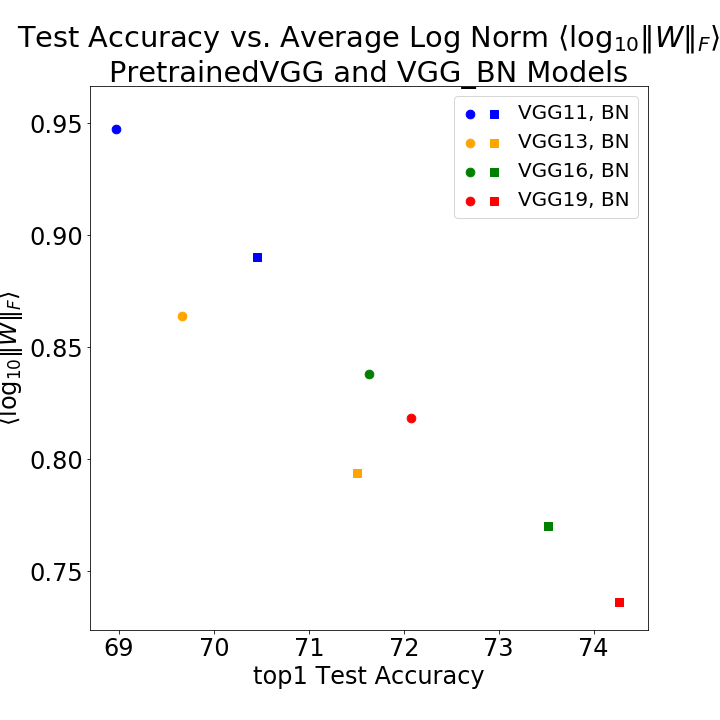
\includegraphics[scale=0.25]{img/vgg-lognorms.png}
      \label{fig:vgg_lognorms}
   }
   \subfigure[weighted average PL exponent $\hat{\alpha}$]{
      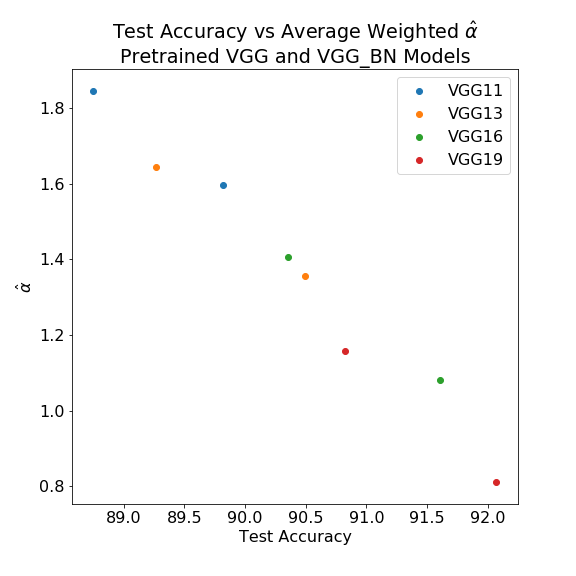
\includegraphics[scale=0.25]{img/vgg-w_alphas.png}
      \label{fig:vgg_alphahat}
   }
   \caption{%
      Pre-trained VGG and VGG\_BN Architectures and DNNs.  
      Top 1 Test Accuracy versus
      average log Frobenius norm $\langle\log\Vert\mathbf{W}\Vert_{F}\rangle$ (in (\ref{fig:vgg_lognorms}))
      or
      Universal, weighted average PL exponent $\hat{\alpha}$ (in (\ref{fig:vgg_alphahat}))
      for
      VGG11 vs VGG11\_BN ({\color{blue}{blue}}),
      VGG13 vs VGG13\_BN ({\color{orange}{orange}}),
      VGG16 vs VGG16\_BN ({\color{green}{green}}),  and
      VGG19 vs VGG19\_BN ({\color{red}{red}}). 
      We plot plain the VGG models with circles and the VGG\_BN models with~squares.
   }
   \label{fig:vgg}
\end{figure*}


%% COMBINED WITH ABOVE %% \begin{figure}[!htb]
%% COMBINED WITH ABOVE %%  \centering
%% COMBINED WITH ABOVE %%    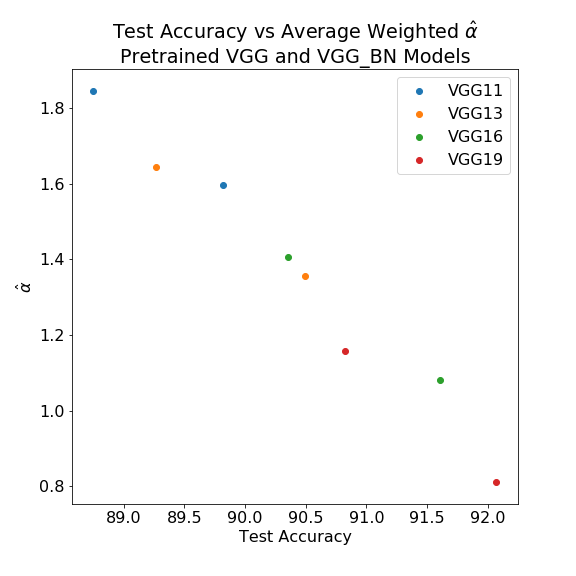
\includegraphics[scale=0.40]{img/vgg-w_alphas.png}
%% COMBINED WITH ABOVE %%    \caption{
%% COMBINED WITH ABOVE %% Pre-trained VGG and VGG BN Architectures and DNNs.  Test Accuracy and weighted average $\hat{\alpha}$ for
%% COMBINED WITH ABOVE %%  VGG11 vs VGG11\_BN ({\color{blue}{blue}}),
%% COMBINED WITH ABOVE %% VGG13 vs VGG13\_BN ({\color{orange}{orange}}),
%% COMBINED WITH ABOVE %% VGG16 vs VGG16\_BN ({\color{green}{green}}),  and
%% COMBINED WITH ABOVE %% VGG19 vs VGG19\_BN ({\color{red}{red}}). 
%% COMBINED WITH ABOVE %% }
%% COMBINED WITH ABOVE %%   \label{fig:vgg_alphahat}
%% COMBINED WITH ABOVE %% \end{figure}



\begin{table}[t]
\small
\begin{center}
\begin{tabular}{|p{0.75in}|c|c|c|c|c|c|c|}
\hline
Model & Top1 Accuracy & $\hat{\alpha}$ \\
\hline
VGG11 & 68.97 & 1.84 \\
VGG11\_BN & 70.45 & 1.60 \\
\hline
VGG13 & 69.66 & 1.65 \\
VGG13\_BN & 71.51 & 1.36 \\
\hline
VGG16 & 71.64 & 1.41 \\
VGG16\_BN & 73.52 & 1.08 \\
\hline
VGG19 & 72.08 & 1.16 \\
VGG19\_BN & 74.27 & 0.81 \\
\hline
\end{tabular}
\end{center}
\caption{%
         Results for VGG Architecture.   The Top1 Accuracy is defined
as the $100.0$ minus the Top1 reported error.
         }
\label{table:models_VGG}
\end{table}


We first look at the VGG class of models, comparing the log norm and the Universal $\hat{\alpha}$ metrics.
See Figure~\ref{fig:vgg} and Table~\ref{table:models_VGG} for a summary of the results.
Figures~\ref{fig:vgg_lognorms} and~\ref{fig:vgg_alphahat} show both the average log Frobenius norm, $\langle\log\Vert\mathbf{W}\Vert_{F}\rangle$ of Eqn.~(\ref{eqn:av_log_norm}), and the weighted average PL exponent, $\hat{\alpha}$ of Eqn.~(\ref{eqn:alpha_hat_specific}), as a function of the reported (Top1) test accuracy for the series of pre-trained VGG models, as available in the pyTorch package.%
\footnote{\url{https://pytorch.org/}}
These models include VGG11, VGG13, VGG16, and VGG19, as well as their more accurate counterparts with Batch Normalization, VGG11\_BN, VGG13\_BN, VGG16\_BN and VGG19\_BN. 
%See Figures~\ref{fig:vgg_lognorms} and~\ref{fig:vgg_alphahat} as well as Table~\ref{table:models_VGG} for details.
Table~\ref{table:models_VGG} provides additional details.

%Figure~\ref{fig:vgg_lognorms} shows the average log Frobenius norm results, which are quite good; and 
%Figure \ref{fig:vgg_alphahat} shows the weighted average PL exponent results, which yield slight improvements due to the method we introduce.
Across the entire series of architectures, 
reported test accuracies increase linearly as each metric, 
%%the average log Frobenius norm 
$\langle\log\Vert\mathbf{W}\Vert_{F}\rangle$
%%, Eqn.~(\ref{eqn:av_log_norm}), 
and 
%%the average weighted power law exponent 
$\hat{\alpha}$,
%%, Eqn.~(\ref{eqn}).
decreases.
Moreover, whereas the log norm relation has 2 outliers, VGG13 and VGG13\_BN, the Universal $\hat{\alpha}$ metric shows a near perfect linear relation across the entire VGG~series.

\paragraph{ResNet Models.}

\begin{figure*}[!htb]
   \centering
   \subfigure[log Frobenius norm $\langle\log\Vert\mathbf{W}\Vert_{F}\rangle$]{
      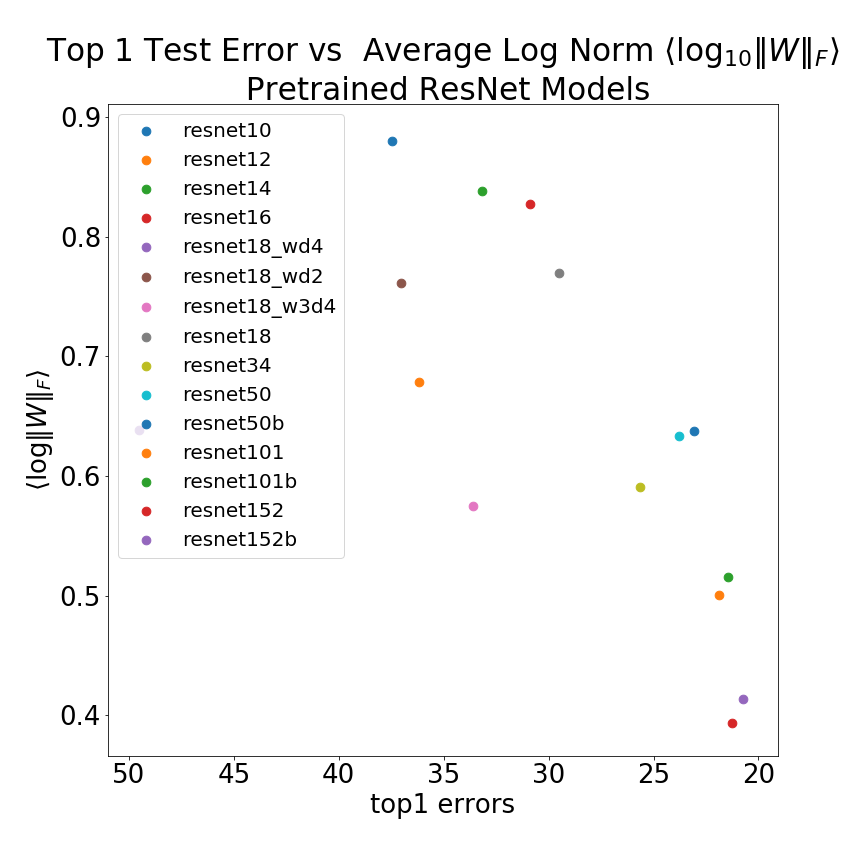
\includegraphics[scale=0.21]{img/ResNet_top1-lognorms.png}
      \label{fig:resnet_lognorms}
   }
   \subfigure[weighted average PL exponent $\hat{\alpha}$]{
      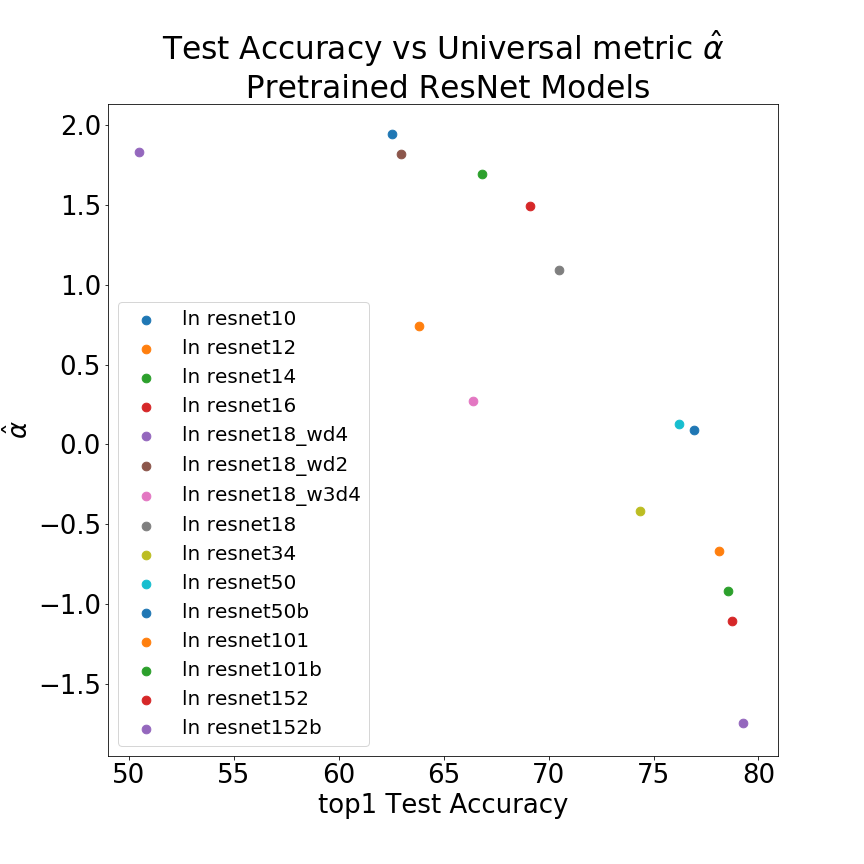
\includegraphics[scale=0.21]{img/ResNet-w_alphas.png}
      \label{fig:resnet_alphahat}
   }
   \caption{
      Pre-trained
      ResNet Architectures and DNNs.  
      Top 1 Test Accuracy versus
      average log Frobenius norm $\langle\log\Vert\mathbf{W}\Vert_{F}\rangle$ (in (\ref{fig:resnet_lognorms}))
      or
      Universal, weighted average PL exponent $\hat{\alpha}$ (in (\ref{fig:resnet_alphahat})).
           }
   \label{fig:resnet}
\end{figure*}

\begin{table}[t] %[!htb]
\small
\begin{center}
\begin{tabular}{|p{0.75in}|c|c|c|c|c|c|c|}
\hline
Architecture 
 & Model
 & Top 1 Accuracy & $\hat{\alpha}$ \\
\hline
ResNet (small)   & resnet10 & 62.54 & 1.94 \\
 & resnet12 & 63.82 & 0.74 \\
 & resnet14 & 66.83 & 1.70 \\
 & resnet16 & 69.10 & 1.49 \\
 \hline
 ResNet18  & resnet18\_wd4 & 50.50 & 1.83 \\
 & resnet18\_wd2 & 62.96 & 1.82 \\
 & resnet18\_w3d4 & 66.39 & 0.28 \\
 & resnet18 & 70.48 & 1.09 \\
 \hline
ResNet34 & resnet34 & 74.34 & -0.42 \\
\hline
ResNet50  & resnet50 & 76.21 & 0.13 \\
 & resnet50b & 76.95 & 0.09 \\
 \hline
ResNet101 & resnet101 & 78.10 & -0.67 \\
 & resnet101b & 78.55 & -0.92 \\
\hline
ResNet152 & resnet152 & 78.74 & -1.11 \\
 & resnet152b & 79.26 & -1.74 \\
\hline
\end{tabular}
\end{center}
\caption{Results for ResNet Architectures and DNN Models.  The Top1 Accuracy is defined
as the $100.0$ minus the Top1 reported error.  Some $\hat{\alpha}<0$ because the of how
the ResNet weight matrices are internally scale and normalized, which makes the maximum eigenvalue
less then one, $\lambda^{max}<1$.
        }
\label{table:models_resnet}
\end{table}


\vspace{-1mm}

We next look at the ResNet class of models. 
See Figure~\ref{fig:resnet} and Table~\ref{table:models_resnet} for a summary of the results.
Here, we consider a set of 15 different pre-trained ResNet models, of varying sizes and accuracies, ranging from the small ResNet10 up to the largest ResNet152 models, as provided by the OSMR sandbox,%
\footnote{\url{https://github.com/osmr/imgclsmob}}
developed for training large-scale image classification networks for embedded systems.
Again, we compare the reported (Top1) test accuracy versus the average log norm $\langle\log\Vert\mathbf{W}\Vert_{F}\rangle$ and the Universal $\hat{\alpha}$ metrics. 

As with the VGG series, both metrics monotonically decrease as the test accuracies decrease for the ResNet series, and both metrics have a few large outliers off the main line relation. 
See Figures~\ref{fig:resnet_lognorms} and~\ref{fig:resnet_alphahat}.
In particular, the log norm metric has several notable outliers, including resnet18\_wd2, resnet18\_wd3\_d4, resnet34, and resnet10. 
The $\hat{\alpha}$ metric shows a slightly better relation, with resnet18\_wd2 more in line, and the other 3 outliers a little less off the main line of correlation. 
The Universal $\hat{\alpha}$ metric is as good or slightly better than the average log norm metric for the Resnet series of models. 

We see similar results for our Universal PL capacity control metric $\hat{\alpha}$ across a wide range of other pre-trained DNN models, described in Appendix~\ref{sxn:appendix-addl-empirical}.
In nearly all cases, the metric $\hat{\alpha}$ correlates well with the reported test accuracies, with only a three DNN architectures as exceptions. 
Overall the $\hat{\alpha}$ metric systematically correlates well with the generalization accuracy of a wide class of pre-trained DNN architectures---which is rather remarkable.

